\chapter{Especificação do Sistema desenvolvido} \label{cap:cap4}

O sistema desenvolvido a partir do uso do dispositivo háptico para treinamento de anestesia raquidiana apresentado nesta tese envolve a criação de um simulador que permite o treinamento de aprendizes na técnica de anestesia raquidiana utilizando um ambiente virtual de treinamento com uso de \acrshort{RV}. Usuários em treinamento recebem \textit{feedback} em relação a execução do procedimento. Foi desenvolvida a modelagem 3D de um tronco de grávida parametrizado de forma a permitir múltiplas variações de cenários de treinamento no que diz respeito as características físicas da paciente. Os experimentos foram executados em três fases com objetivos distintos. A primeira para testar a viabilidade de representação das principais sensações envolvidas neste tipo de anestesia. Nesta fase gráficos de força \textit{versus} deslocamento da agulha foram utilizados para descrever o comportamento durante a perfuração das camadas nos experimentos desta tese. Também foram usados questionários onde procurou-se reduzir a subjetividade da interpretação dos gráficos. Na segunda fase de testes o objetivo foi a avaliação da usabilidade do sistema e para tal foi utilizado o método SUS \cite{Brooke2013}. Na terceira e última fase foram feitos testes com especialistas visando validar a assertividade das representações das sensações em comparação com o procedimento real bem como traçar um comparativo com um simulador com características similares.

O ambiente virtual desta tese foi desenvolvido utilizando o motor de jogo Unity3D \cite{UnityTechnologies2020} com uso de \textit{plugin} para o dispositivo háptico \textit{Geomagic Touch}®, os \textit{scripts} foram desenvolvidos em C\#. O código foi desenvolvido tomando como ponto de partida o simulador epidural desenvolvido por \textcite{Brazil2017thesis}. Diversas funcionalidades existentes foram estendidas e modificadas bem como outras foram criadas ou removidas de acordo com a necessidade. 
O foco passou de anestesia epidural para anestesia raquidiana. Um novo modelo 3D foi construído para representar as camadas do corpo humano, para isto, as formas e volumes das camadas foram baseadas num corpo 3D interativo cientificamente preciso \cite{BioDigitalInc2019}. Adicionalmente, as principais camadas (tecidos do corpo) foram programadas com uma margem de crescimento individual onde o crescimento da camada mais interna ``empurra'' as camadas mais externas pra fora. Isto foi feito para possibilitar uma maior diversidade de cenários e para que estes sejam visualmente coerentes quando a transparência das camadas for aplicada. Além da possibilidade de se crescer individualmente cada camada, também é possível que todas as camadas cresçam de forma homogênea através da aplicação de matrizes de transformação. 

\section {Desenvolvimento do ambiente de treinamento} 
\label{sec:desenvolvimentoAmbienteTreinamento}

O modelo 3D para o tronco do corpo feminino (área onde é feita a punção) foi desenvolvido usando o software de modelagem e criação \textit{3ds Max} \cite{Autodesk}. Exemplos das suas diversas camadas internas podem ser observados na Figura \ref{fig:modelo3Dcorpo}. 

\begin{figure}[ht!]
    \centering
        \begin{tabular}{cc}
        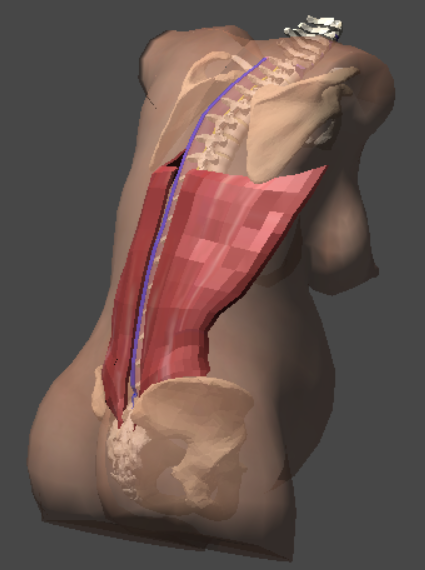
\includegraphics[width=0.4\linewidth]{capitulos/figuras/modelo corpo 3d.PNG} & 
        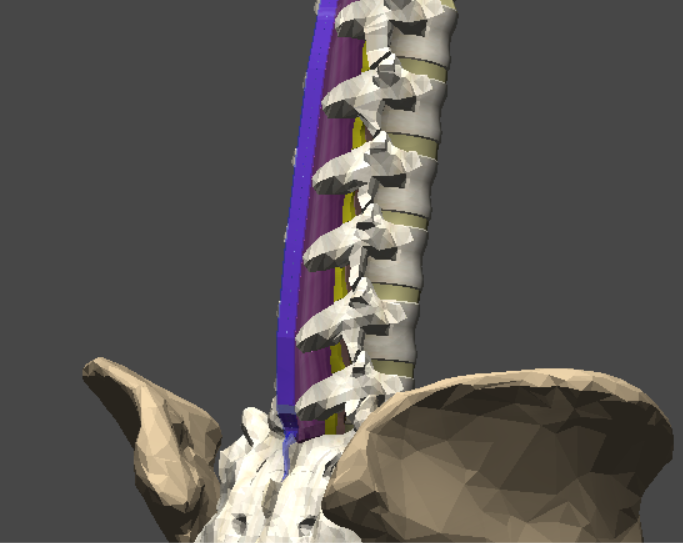
\includegraphics[width=0.5\linewidth]{capitulos/figuras/modelo corpo 3d - coluna vertebral, ligamentos supra, interespinhoso and flavum.PNG} 
        \\
        (a) & (b)
        \end{tabular}
    \caption{Modelo 3D de corpo de mulher grávida desenvolvido com diferentes níveis de transparência \cite{Melo2021}: (a) Corpo, ossos e músculos (b) Osso, vértebras e ligamentos.}
    \label{fig:modelo3Dcorpo}
\end{figure}

Como comentado anteriormente foram criados controles para crescimento das principais camadas do corpo. Para seu uso, primeiro é necessário iniciar um projeto na \textit{Unity} e importar o modelo 3D. Com isto estes controles ficam acessíveis via código nas diversas linguagens suportadas pela \textit{Unity} assim como via interface da \textit{Unity}. Como foi necessário fazer modificações em tempo de execução optou-se pelo acesso através do código em C\# para fazer as modificações de tamanho das camadas (quando necessário). 

Para que seja possível fazer a interação com o dispositivo háptico \textit{Geomagic Touch®} o driver \textit{Open Haptics Touch Device} precisa ser instalado na máquina onde o dispositivo será usado, este driver pode ser encontrado no endereço eletrônico da empresa responsável pela produção e comercialização deste dispositivo háptico \cite{3DSystemsTouch2018}. Para que este dispositivo possa ser utilizado na \textit{Unity} isto foi feito através da instalação do \textit{Haptic Plug-In For Unity3D} \cite{Poyade2014}. Este \textit{plugin} contém exemplos que exploram as funcionalidades dos dispositivos hápticos suportados. As características específicas que foram utilizadas nos experimentos são comentadas no Capítulo~\ref{cap:cap5}. No ambiente de treinamento foram utilizadas configurações levando em consideração o retorno dos experimentos ajustadas de acordo com cada corpo de paciente em simulação. 

Foi incluída uma visão lateral (Figura~\ref{fig:posicaoSentadaComTransparencia}) para possibilitar um outro ponto de vista do procedimento (ideia oriunda do \textit{feedback} de um anestesista sobre pontos de melhoria da ferramenta de treinamento). Esta característica ajuda não só o indivíduo em treinamento mas também pessoas que estejam assistindo ao vivo ou ainda gravações deste que venham a ser disponibilizadas futuramente. Nesta mesma imagem também é possível observar a demonstração da visibilidade das camadas interiores do corpo (que é exibida ao pressionar com o mouse o botão ``visibilidade'' no menu do lado esquerdo) ou ao pressionar a tecla ``V'' do teclado. Esta funcionalidade pode ser utilizada por iniciantes nos seus primeiros treinamentos assim como por educadores para turmas que estejam assistindo demonstrações feita por estes. Pode-se ler ainda nessa imagem (no alto à direita) as instruções sobre como alternar entre equipamentos, essa alteração pode ser feita a partir de números do teclado ou do segundo botão do dispositivo háptico. Foi considerado aqui como primeiro botão o botão que fica mais perto da ponta da ``caneta'' do dispositivo. Este primeiro botão ao ser pressionado faz com que o líquido da anestesia seja expelido da seringa. As setas para direita e esquerda variam a posição de visualização como se o médico estivesse se deslocando lateralmente na cena. Na parte da esquerda (ligeiramente acima da área do tronco da paciente) e acima dos botões estão os dados da paciente (idade, altura e peso). 

\begin{figure}[ht!]
    \centering
    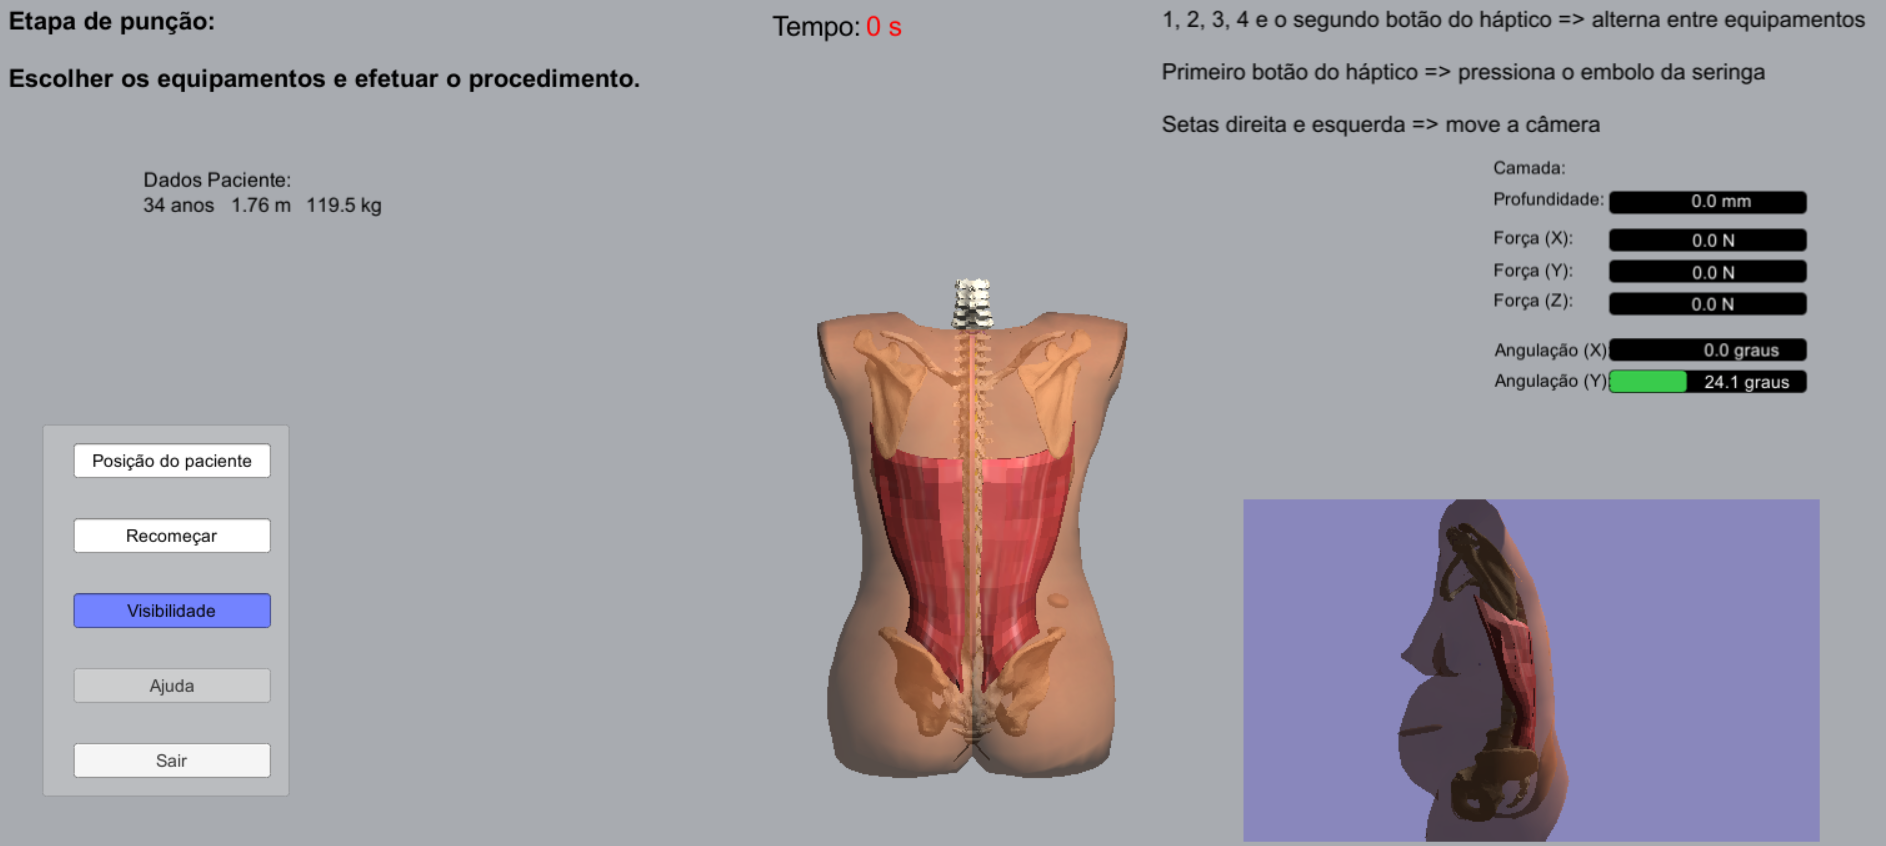
\includegraphics[width=0.9\linewidth]{capitulos/figuras/sistema posicao sentada com transparencia.png} 
    \caption{Visão geral do sistema com tronco de paciente centralizada na tela na posição sentada. Do lado inferior direito a visão lateral desta mesma parte do corpo. Neste caso foi aplicada a transparência para visualização das camadas internas}
    \label{fig:posicaoSentadaComTransparencia}
\end{figure}

Uma outra opção de execução do procedimento incluída foi a possibilidade de mudança de posição da paciente (Figura~\ref{fig:posicaoDeitada}) que além da posição sentada (forma inicial escolhida para o simulador) agora também permite que o procedimento seja feito com ela deitada (estas são as duas posições em que ocorre o procedimento de raquianestesia conforme descrito na Seção \ref{sec:anestesiaRaquidiana}).

\begin{figure}[ht!]
    \centering
    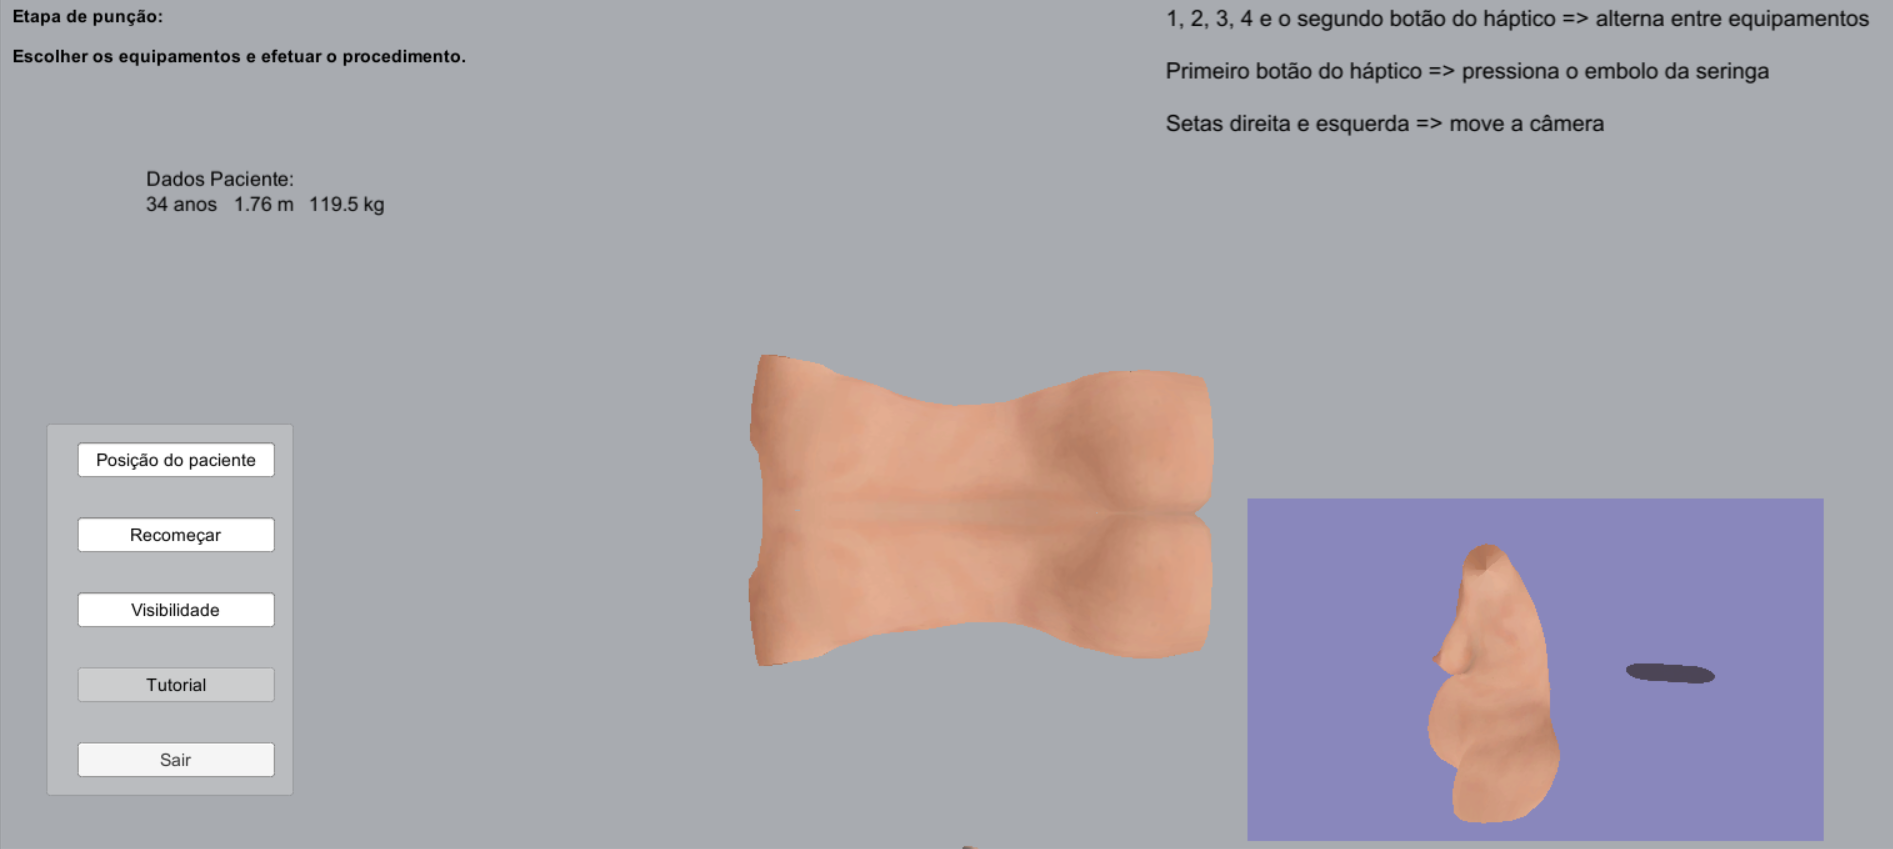
\includegraphics[width=0.9\linewidth]{capitulos/figuras/sistema posicao deitada.png} 
    \caption{Visão geral do sistema com tronco de paciente na posição deitada.}
    \label{fig:posicaoDeitada}
\end{figure}

\subsection {Simulação de pacientes virtuais} 
\label{sec:SimulacaoPacientesVirtuais}

Um dos benefícios da criação de ambientes virtuais para treinamento é a possibilidade de se ter uma quantidade muito grande de casos com características diferentes para o treinamento. Estas possibilidades estão limitadas somente pela abrangência do modelo para criação de pacientes virtuais. Conforme descrito anteriormente para esta tese foi criado e utilizado um modelo dinâmico para geração de pacientes do sexo feminino grávidas. A variação física externamente visível das pacientes é função da altura e massa corpórea. Para as camadas internas envolvidas na anestesia raquidiana a distância da pele até o espaço epidural (\acrshort{DEE}) também entra nessa conta para uma representação mais real da relação entre os dados de massa e altura da paciente com a distância entre estas camadas conforme descrito na Seção \ref{sec:modelagemTecidos}. 

Nesta Seção descreve como foram usados os dados e equações de populações locais descritas por \textcite{Clinkscales2007, Sharma2011, Hazarika2016} para a modelagem de uma equação genérica na determinação da \acrshort{DEE} buscando representar todos os grupos populacionais da Tabela~\ref{tab:PopulacaoPorEstudo}.
A abordagem que detalhada aqui foi descrita em trabalho publicado por nós \cite{Melo2020}.

\textcite{Sharma2011} ao invés das equações apresentaram cinco pontos contendo a \acrshort{DEE} o \acrshort{IMC} representando cada população, optou-se então por utilizar o método dos mínimos quadrados para obter as equações de cada grupo através do melhor ajuste de curva que representasse cada um dos quatro grupos da Tabela~\ref{tab:DEEEstimadosSharma}. Para cada ponto o eixo X representa \acrshort{IMC} e o eixo Y a \acrshort{DEE}. As equações resultantes (que minimizam a soma do quadrado das diferenças para cada ponto) para cada grupo desta tabela estão representadas na Tabela~\ref{tab:DEEEquacoesMinimosQuadrados}. Os nomes dos grupos na tabela estão renomeados para a forma que estes serão referenciados no restante desta tese.

\begin{table}[!ht]
\begin{center}
\caption{Equações resultantes do uso do métodos dos mínimos quadrados nos dados de \textcite{Sharma2011}.}
\label{tab:DEEEquacoesMinimosQuadrados}
\begin{tabular}{|p{0.4\linewidth}|p{0.4\linewidth}|}
\hline
\textbf{Grupo} & \textbf{Equação}\\
\hline\hline
RU - Brancas & DEE = 2,18 + 0,13 IMC\\
RU - Asiáticas & DEE = 2,24 + 0,11 IMC\\
RU - Negras & DEE = 1,98 + 0,15 IMC\\
RU - Chinesas & DEE = 3,08 + 0,07 IMC\\
\hline
\end{tabular}
\end{center}
\end{table}

Os dados brutos dos indivíduos de cada população dos três trabalhos analisados na Seção \ref{sec:modelagemTecidos} não foram disponibilizados publicamente. Desta forma, foi tomado como premissa que o resultado de cada equação representa corretamente a \acrshort{DEE} dos indivíduos da população para o qual cada trabalho foi desenvolvido. Com isto foram gerados randomicamente dados de massa, altura e idade para duzentas pacientes. Os valores mínimos e máximos para cada parâmetro foram: Massa (em quilos) de 50 a 70; Altura (em metros) de 1,40 a 1,90; Idade de 18 a 40 anos. Os valores de massa e altura foram utilizados para que fossem contemplados indivíduos com baixo peso, peso médio, sobrepeso e obesidade com base na \textit{Pregnancy Weight Gain Calculator} (Calculadora de ganho de peso na gravidez) \cite{MTILLC2019}. Pra idade mínima foi levada em conta a definição de maioridade civil e para a idade máxima foi considerado o aumento do risco de gravidez acima da idade de quarenta anos. A quarta variável de entrada, \acrshort{IMC}, foi calculada pela equação padrão (que usa massa em quilos dividido pelo quadrado da altura em metros).  A Tabela~\ref{tab:DadosPopulacaoGerada} descreve a média e o desvio padrão das três características das pacientes que foram geradas randomicamente para criar os dados populacionais assim como o \acrshort{IMC} calculado a partir destas três variáveis. 

\begin{table}[!ht]
\begin{center}
\caption{Dados populacionais gerados aleatoriamente.}
\label{tab:DadosPopulacaoGerada}
\begin{tabular}{|p{0.3\linewidth}|p{0.2\linewidth}|p{0.3\linewidth}|}
\hline
\textbf{Característica} & \textbf{Média} & \textbf{Desvio Padrão}\\
\hline\hline
Idade (anos) & 28,70 & 6,58\\
Altura (m) & 1,65 & 0,15\\
Massa (kg) & 68,97 & 11,80\\
IMC ($kg/m^2$) & 25.84 & 6,55\\
\hline
\end{tabular}
\end{center}
\end{table}

Usando os dados populacionais como entrada foi calculado o \acrshort{DEE} das duzentas pacientes para cada grupo populacional usando as equações das Tabelas \ref{tab:equacoesEstimativaDEE} e~\ref{tab:DEEEquacoesMinimosQuadrados}. A Figura~\ref{fig:mediaDesvioPadraoPopulacoes} ilustra as médias e desvios padrões da \acrshort{DEE} dos grupos populacionais sinteticamente gerados a partir das equações destas tabelas. No gráfico desta figura cada grupo é identificado pelo local de onde  foram feitos os estudos que geraram as equações ou os dados que embasaram as equações para produção das amostras sintéticas assim como pelos grupos nos quais cada estudo separou seus dados.

\begin{figure}[ht!]
    \centering
    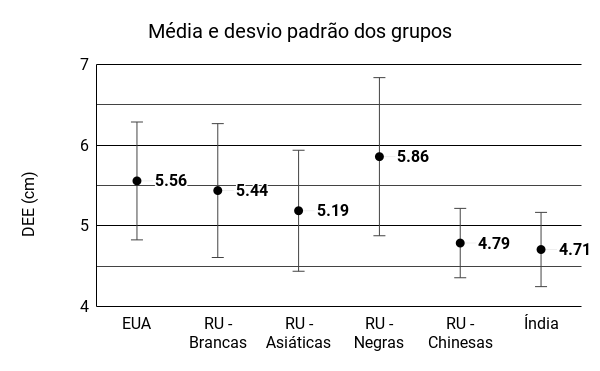
\includegraphics[width=0.8\linewidth]{capitulos/figuras/Media e desvio padrao dos grupos.png} 
    \caption{Média e desvio padrão da \acrshort{DEE} estimada para as populações de cada grupo de grávidas separadas pelo local dos estudos e grupos distintos.}
    \label{fig:mediaDesvioPadraoPopulacoes}
\end{figure}

Para determinação de uma equação geral foram considerados os dados de todos os indivíduos em um grande conjunto. Os dados de todos os seis grupos foram utilizados como entrada de um método de regressão multilinear sem levar em consideração os grupos populacionais. A amostra populacional randômica é de n=200 (número de indivíduos em cada grupo), considerando os 6 grupos tem-se então uma população para esta abordagem de n=1200. A influência de todas as variáveis  independentes (massa, altura, idade e \acrshort{IMC}) foi testada em relação à \acrshort{DEE} no modelo de regressão multilinear. Somente o \acrshort{IMC} demonstrou ter significância estatística (p<0,01). A equação de regressão \ref{equ:equacaoGenerica} representa este modelo. 

\begin{equation}
\label{equ:equacaoGenerica}
Y=2,52+0,11 IMC
\end{equation}

Levando em consideração os dados de todos os grupos, o valor médio da \acrshort{DEE} é de 5,3 cm com um desvio padrão de 0,74 cm. Os valores mínimos e máximos são respectivamente 3,82 cm e 8,6 cm. A Figura~\ref{fig:imcDEEPopulacoesComparativoEquacaoGenerica} mostra graficamente a comparação dos resultados das estimativas da  \acrshort{DEE} para as equações de todos os grupos em relação à equação genérica (curva laranja). O grupo de nome ``RU - Negras'' apresenta os maiores valores de \acrshort{DEE} e o grupo Índia e ``RU - Chinesas'' apresentam os valores mais baixos. Os resultados da equação genérica apresentam como resposta um valor médio de todos os grupos.

\begin{figure}[ht!]
    \centering
    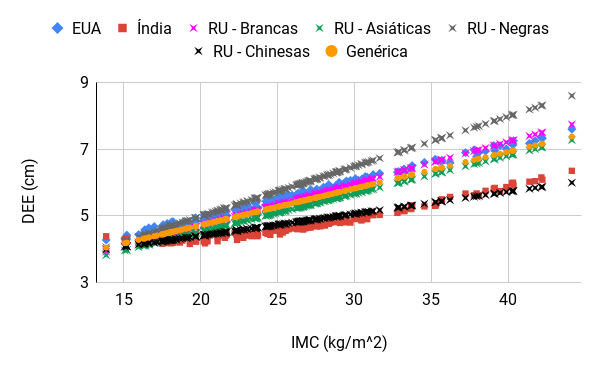
\includegraphics[width=0.9\linewidth]{capitulos/figuras/IMC versus DEE grupos populacionais e Equacao Generica.png} 
    \caption{\acrshort{IMC} x \acrshort{DEE} para os grupos populacionais em comparação a equação genérica.}
    \label{fig:imcDEEPopulacoesComparativoEquacaoGenerica}
\end{figure}

O valor 69,19\% do R-quadrado ajustado se refere a equação \ref{equ:equacaoGenerica}. Este valor indica a proximidade entre os valores observados e estimados da variável analisada (neste caso a \acrshort{DEE}). É um indicativo de quanto o modelo de regressão se aproximou dos dados de entrada. Embora o foco desta tese seja na representação da realidade brasileira é importante ressaltar que não foram encontradas nas nossas pesquisas dados deste tipo para a população brasileira que é conhecidamente uma população miscigenada.  Com uma aproximação de quase 70\% e representando uma média das diferentes populações usadas como entrada para este cálculo foi assumido que a equação genérica pode ser satisfatória para fins de determinação da \acrshort{DEE} de brasileiras por ter sido estimada a partir de uma população diversa e abrangente. Esta equação foi portanto utilizada nesta tese por não existirem equações mais representativas da determinação deste valor para grávidas brasileiras que é o foco aqui.

Para a determinação do tamanho de cada camada foi utilizada então o valor da \acrshort{DEE} calculada por essa equação genérica fazendo com que o crescimento seja proporcional em cada camada. Dessa forma esse crescimento mantém a ordem de grandeza dos tamanhos das camadas e leva em conta a informação de que o tecido mais afetado com a variação do \acrshort{IMC} do paciente provavelmente deve se relacionar a gordura subcutânea \cite{Palmer1983}.

A seguir é ilustrado como considerar a possibilidade de variação ou criação de novos corpos de pacientes através dos parâmetros existentes no modelo 3D desenvolvido. Essas alterações do corpo podem ser feitas tanto via interface da \textit{Unity} (de forma estática) como via código C\# (de forma dinâmica). 

Como primeiro exemplo são apresentadas as alterações de crescimento do tronco simulando uma paciente com um \acrshort{IMC} mais elevado em comparação com uma paciente com um corpo de \acrshort{IMC} mais baixo. As duas imagens apresentadas na Figura~\ref{fig:extremosCorpoIMC} ilustram os extremos que podem ser obtidos com a variação de parâmetros implementada no modelo 3D criado. Para variações maiores é possível usar transformações matriciais através de simples comandos na \textit{Unity} usando a transformação de escala aplicados. Nesta tese optou-se pela implementação de um range de variação para evitar a deformação através de matrizes de transformação aplicadas no objeto 3D como um todo. É sabido que existem regiões que são as mais afetadas pelo ganho de gordura corporal e, portanto, devem ser mais expandidas do que outras, visando um ganho visual mais próximo do real. A Figura~\ref{fig:extremosCorpoIMC} apresenta o \textit{wireframe} de forma a ilustrar os polígonos que fazem parte do modelo 3D do corpo. Para fazer essas alterações via interface da \textit{Unity} primeiro é necessário importar o modelo 3D no projeto. Em seguida é necessário adicionar este a hierarquia e posicioná-lo corretamente na cena. Ao selecionar o elemento do modelo 3D (que se chama \textit{Body}) é preciso alterar o componente \textit{Skinned Mesh Renderer} associado pelo \textit{Unity} no momento da importação para cada camada (parte do modelo 3D) que possui parametrização (os componentes ficam na janela \textit{Inspector}). Este componente possui uma Seção chamada \textit{BlendShapes} que exibe os parâmetros de deformação da forma. O parâmetro do objeto \textit{Body} se chama \textit{Body\_Final\_Channel} e aceita valores de zero a cem, sendo 0 (zero) o valor que indica a ausência de deformação (Figura~\ref{fig:extremosCorpoIMC} (a)) e 100 (cem) o valor de maior deformação (Figura~\ref{fig:extremosCorpoIMC} (b)). Para alteração via código na mudança de pacientes foi utilizado o script em C\#. O acesso para modificação deste percentual de deformação é feito a partir da variável que representa o corpo, para este caso a camada \textit{Body} fica posicionada num vetor de camadas na primeira posição. A Listagem~\ref{lst:codigo_alteracao_forma_paciente} apresenta um exemplo da parte do código que faz a deformação do corpo do paciente a partir do parâmetro passado. Este parâmetro é calculado como valor percentual a partir dos valores de \acrshort{DEE} mínima e máxima implementados no sistema e do \acrshort{IMC} do paciente que é calculado a partir do seu peso e altura. A equação \ref{equ:equacaoGenerica} foi utilizada para cálculo da \acrshort{DEE} de cada paciente e, portanto, para determinação dos seus mínimos e máximos. Os valores mínimos e máximos da \acrshort{DEE} são fixos pra cada execução do sistema sendo calculados a partir da base de pacientes disponível. Esta base pode ser alterada livremente para aumentar ou diminuir a variabilidade de cenários de teste conforme necessidade.

\begin{lstlisting}[label=lst:codigo_alteracao_forma_paciente, caption={Exemplo de alteração do corpo do paciente via script em C\#.}, language=sharpc]
float imc = objPaciente.peso / (objPaciente.altura * objPaciente.altura);
float dee = 2.52 + 0.11 * imc
float percentDeformacaoCorpo = 100 * (dee - minDEE) / (maxDEE - minDEE);
        
SkinnedMeshRenderer smRenderer;
smRenderer = camadas[0].GetComponent<SkinnedMeshRenderer>();
smRenderer.SetBlendShapeWeight(0, percentDeformacaoCorpo);
\end{lstlisting}

\begin{figure}[ht!]
    \centering
        \begin{tabular}{cc}
        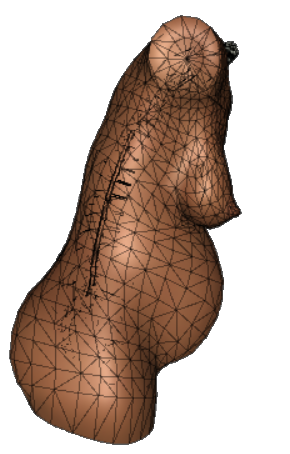
\includegraphics[width=0.4\linewidth]{capitulos/figuras/Corpo-menor-IMC-Wireframe.png} & 
        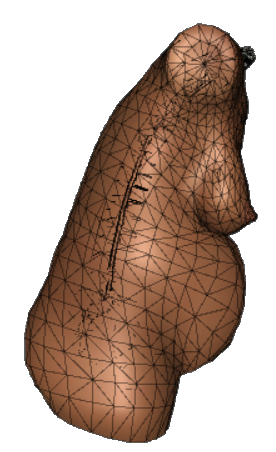
\includegraphics[width=0.38\linewidth]{capitulos/figuras/Corpo-maior-IMC-Wireframe.png} 
        \\
        (a) & (b)
        \end{tabular}
    \caption{Troncos com extremos de \acrshort{IMC} via parâmetro na posição lateral com \textit{wireframe}: (a) Menor \acrshort{IMC} (b) Maior \acrshort{IMC}.}
    \label{fig:extremosCorpoIMC}
\end{figure}

A Figura~\ref{fig:pacientesMaiorParaMenorIMCVisaoTroncoELateral} exibe todas as pacientes atualmente cadastradas no sistema ordenadas de forma decrescente em relação ao \acrshort{IMC}. Ao lado de cada tronco com os dados de idade, altura e peso também é exibida uma visão lateral para melhor visualização das diferenças (que são distribuídas nos eixos X e Z). Fazendo um comparativo desde a paciente com maior \acrshort{IMC} (no alto à esquerda) até a de menor (abaixo à direita) é possível observar parte das variações implementadas no modelo 3D em relação à camada do corpo. Observando a área da cintura, barriga e dorso pode-se perceber o afinamento destas áreas conforme o \acrshort{IMC} é reduzido. É importante ressaltar aqui que a possibilidade de ajustar altura (crescimento no eixo Y) não foi trabalhada no modelo 3D por motivos de simplificação mas esta pode ser alterada a partir de transformações de matrizes que são simplificadas através da classe \textit{Transform} da \textit{Unity}. Na Figura~\ref{fig:alteracaoModeloAltura} é possível ver na imagem central o tronco da paciente na sua escala normal e duas alterações de escala variando somente a altura em vinte porcento para mais (à direita) e para menos (do lado esquerdo). Da mesma forma que as alterações comentadas anteriormente esta também podem ser feita de forma estática ou dinâmica. Ajustes na altura envolvem o aspecto da correspondência com os dados da paciente bem como um leve aumento ou diminuição do espaço entre as vértebras. De toda forma o eixo mais importante para o contexto da simulação de raquianestesia é o da profundidade das camadas a serem transpassadas (eixo Z), por que é neste eixo que a agulha é inserida.

\begin{figure}[ht!]
    \centering
    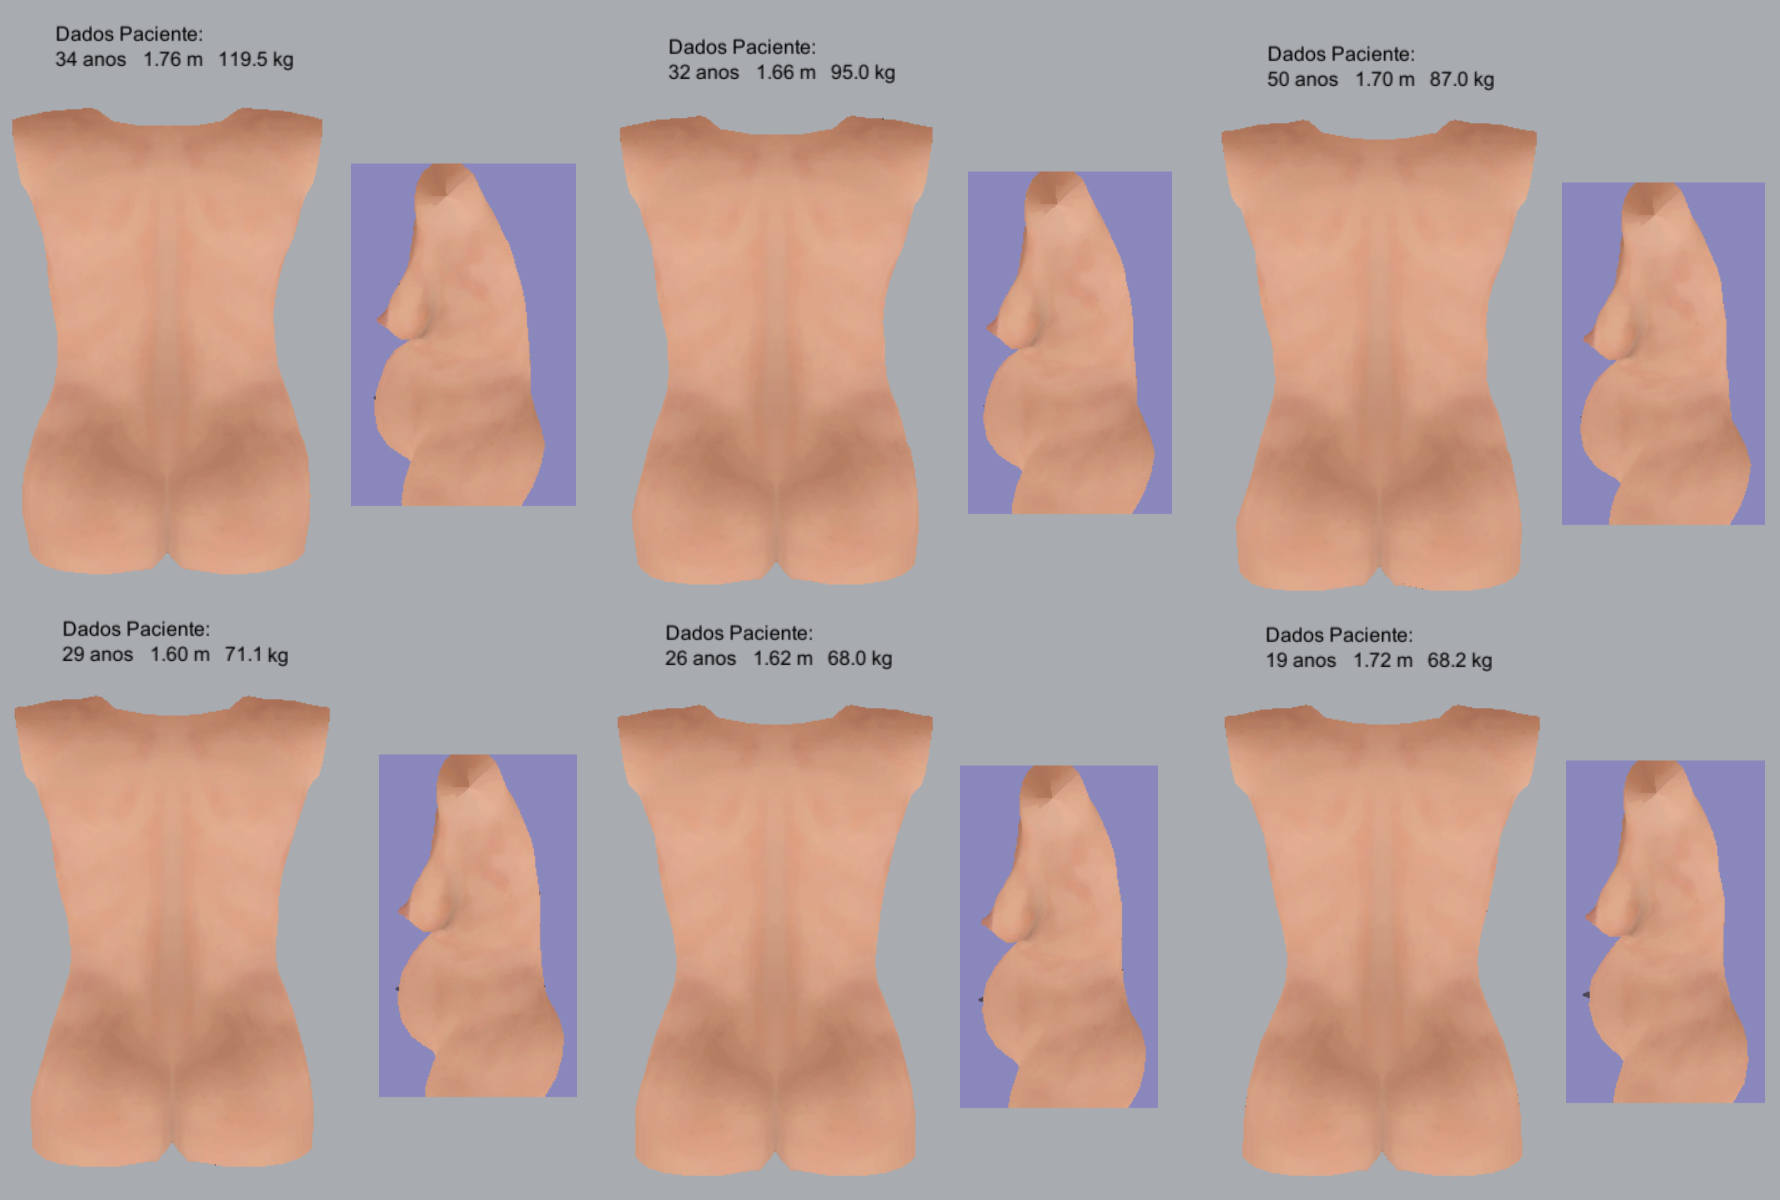
\includegraphics[width=0.9\linewidth]{capitulos/figuras/pacientes cadastradas maior para menor imc visao tronco sentado e lateral.png} 
    \caption{Ilustração dos troncos das pacientes cadastradas renderizados no sistema juntamente com a visão lateral do maior para o menor IMC.}
    \label{fig:pacientesMaiorParaMenorIMCVisaoTroncoELateral}
\end{figure}

\begin{figure}[ht!]
    \centering
    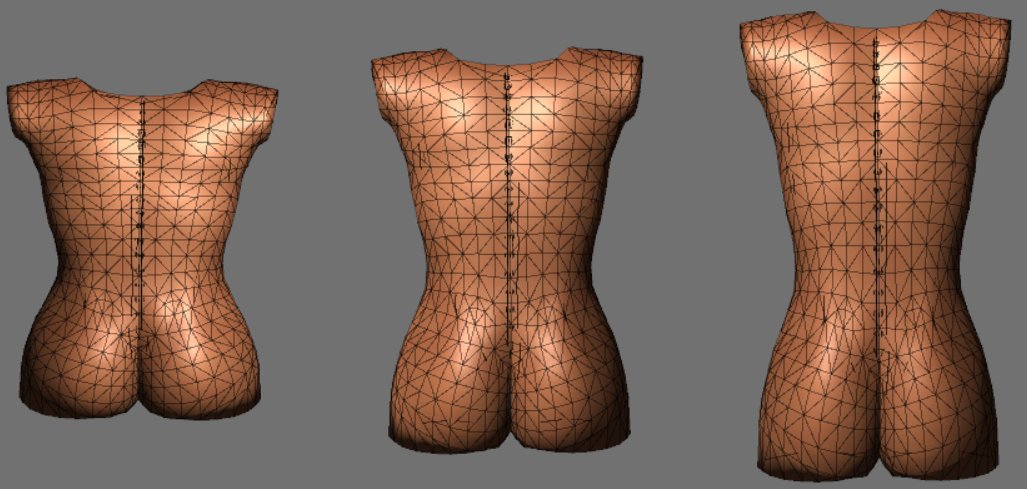
\includegraphics[width=0.9\linewidth]{capitulos/figuras/alteracao-modelo-altura.png} 
    \caption{Exemplos de variação na altura do tronco por alteração em 20\% para mais e para menos.}
    \label{fig:alteracaoModeloAltura}
\end{figure}

Para configuração do \textit{Haptic Plug-In For Unity3D} \cite{Poyade2014}, \textit{plugin} utilizado para tratar a interface entre o dispositivo háptico e os itens 3D da simulação, foi necessário adicionar a cada camada do corpo alguns componentes. Os componentes a serem adicionados às camadas são o \textit{Haptic Properties} e o \textit{Mesh Collider} através da seleção da camada na hierarquia e, em seguida, no \textit{Inspector} deve-se ir no item Adicionar componentes e entrar com o nome destes. O componente \textit{Haptic Properties} vem junto com o \textit{Haptic Plug-In For Unity3D}. Ele serve para configurar as propriedades de interação com o háptico aos itens do universo 3D como as camadas do corpo da paciente no nosso caso (pele e demais camadas internas). Um exemplo de propriedade é a \textit{Pop Through} que indica que força é necessário aplicar para que se perfure cada camada que está em contato com a agulha de anestesia durante uma simulação. Existem então configurações distintas para quando o movimento do háptico está representando o movimento do dedo do anestesista para apalpação e descobrimento do local correto de punção e para o momento que o movimento representa os objetos perfurantes como a seringa de anestesia local e a agulha de raquianestesia. No caso do anestesista estar fazendo a apalpação esta propriedade deve assumir um valor que desabilita a perfuração (o valor para este caso é zero). Esta e demais características a respeito das propriedade utilizadas são descritas no Capítulo~\ref{cap:cap5}. Já o componente \textit{Mesh Collider} é nativo do \textit{Unity} e é uma das formas de detecção de colisão da \textit{engine} que usa a geometria visível do objeto para tal. Outra configuração necessária para todos os objetos que têm interação com o háptico é a inclusão da tag \textit{Touchable} que deve ser feita através do \textit{Inspector}. A tag \textit{Touchable} também deve ser incluída em todos os objetos 3D que podem sofrer alguma influência a partir da movimentação do dispositivo háptico.

% === FALAR sobre associações de scripts Haptic Injection, Generic Functions Class?
